\section{Algoritmos de Classificação}
\label{sec:algoritmos}

Um algoritmo de classificação pode ser definido como uma função que recebe como entrada um conjunto de registros com atributos discretos, incluindo um atributo escolhido como classe, e pesa esses atributos de forma a devolver como saída registros separados em classes. O classificador é treinado para identificar os pesos que resultam na classificação mais precisa, então testado por suas predições de classe.

Estudos anteriores mostram que é difícil encontrar algoritmos de classificação que tenham bom desempenho em qualquer cenário, então é desejável que suas características sejam levadas em consideração ao tentar identificar um algoritmo que traga boas predições ao problema em mãos \cite{gama-algoritmos}.

Então, se baseando nos trabalhos relacionados ao tema, é considerado relevante para o atual estudo analisar o desempenho dos seguintes algoritmos de classificação:

\subsection{k-Nearest Neighbors}
\label{subsec:contexto-knn}

kNN, ou \textit{k-Nearest Neighbors}, é um algoritmo de classificação baseado na ideia de que registros de classes similares ficariam aglomerados quando colocados em um vetor de n-dimensões.

Em um vetor cujas dimensões são definidas pelo número de atributos, todos os registros do conjunto de dados de treinamento são colocados em posições conforme os valores de seus atributos, idealmente próximos a outros registros da mesma classe. Então, na etapa de teste, os registros sem classe têm sua posição definida, e por meio da distância dos seus vizinhos mais próximos, é predita a classe de cada registro. A distância pode ser euclidiana, \textit{Hamming}, \textit{Manhattan} ou qualquer outra distância entre dois vetores, porém a euclidiana é a mais comum, e pode ser calculada com a equação abaixo \cite{knn}.

\begin{equation}
  \text{Distância Euclidiana} = \sqrt{\sum_{i=1}^{n} (x_i - x_j)^2}
  \end{equation}

O número de vizinhos mais próximos é definido pelo parâmetro \textit{k}, que é um valor inteiro positivo, idealmente ímpar de modo a evitar a predição de classes como \"ambas\" quando há um número igual de classes vizinhas. Este valor muitas vezes é escolhido por tentativa e erro, seguindo as métricas de desempenho do algoritmo \cite{knn-medium}.

\begin{figure}[ht!]
  \centering
  \fcolorbox{white}{white}{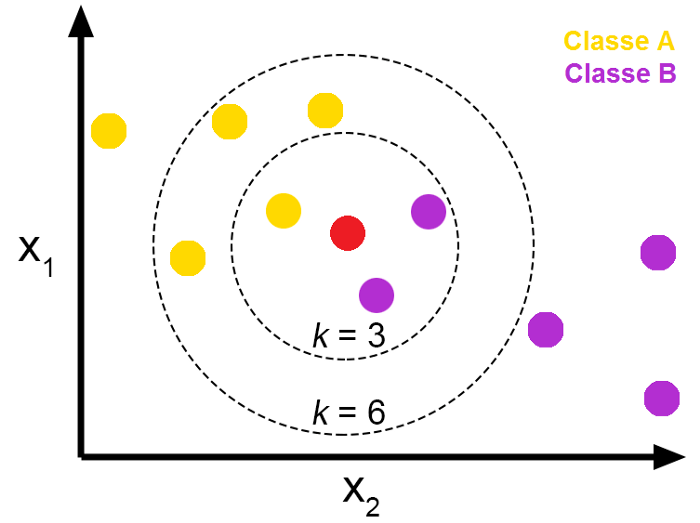
\includegraphics[width=0.5\textwidth]{chapters/contexto/images/knn.png}}
  \caption{\textmd{Exemplo de kNN com k = 3 e k = 6}}
  \legend{Fonte: KNN (K-Nearest Neighbors) \#1 - Italo José (Medium)}
  \label{fig:knn-exemplo}
\end{figure}

Como os valores são utilizados como posição, kNN se beneficia de uma distribuição uniforme de valores para os atributos, sendo importante realizar a normalização e escala dos dados. O algoritmo também é considerado preguiçoso, não tendo uma etapa de treinamento propriamente dita, também tendo baixa eficiência, pois todos os registros são testados pela sua distância, mas costuma ter um desempenho satisfatório em alguns casos \cite{knn-desempenho}.


\subsection{Decision Tree}
\label{subsec:contexto-decision-tree}

\textit{Decision Tree}, ou Árvore de Decisão, é um algoritmo interpretável de classificação que divide o conjunto de dados em subconjuntos, através de critérios de decisão, e a partir desses subconjuntos são criadas novas subárvores, até que todos os registros sejam classificados\cite{dtree}.

Os critérios de decisão são funções que dividem os dados entre Verdadeiro e Falso, a partir de um dos atributos dos registros, por exemplo, criando uma subárvore, ou galho, onde todos os registros têm idade maior ou igual a 60, e um outro galho onde os registros têm idade menor que 60. Essa divisão acontece até que o algoritmo decida que não é mais necessário dividir os subconjuntos, criando uma folha, onde todos os registros são classificados como a mesma classe. Os galhos e folhas também são chamados de \"nós\", sendo a árvore construída a partir de um nó raiz \cite{dtree-explained}.

\begin{figure}[ht!]
  \centering
  \fcolorbox{white}{white}{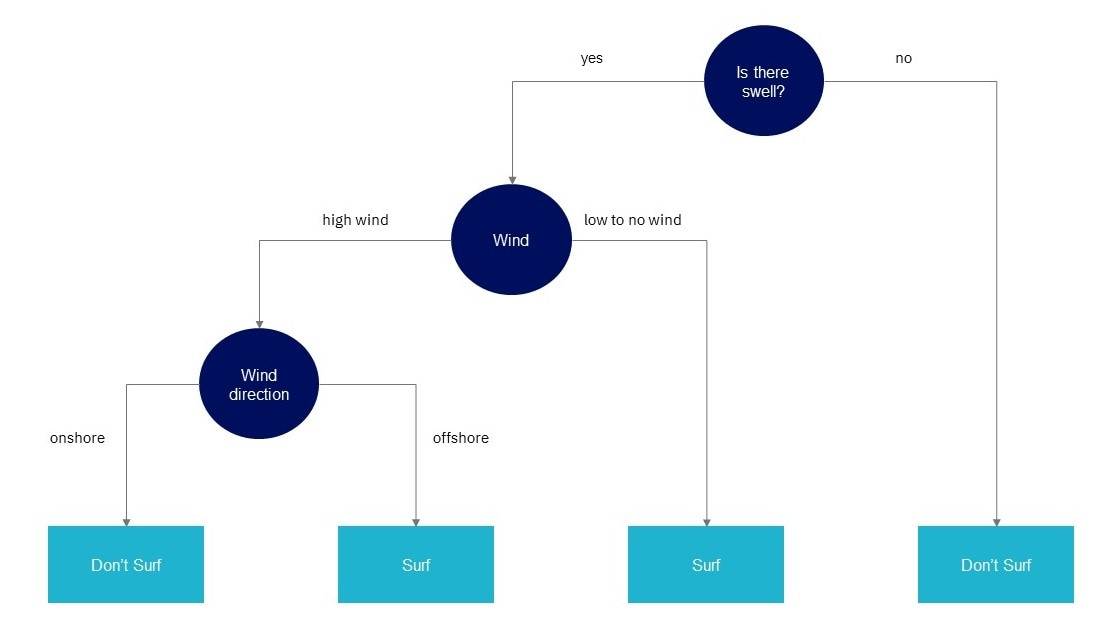
\includegraphics[width=0.5\textwidth]{chapters/contexto/images/dtree.jpg}}
  \caption{\textmd{Exemplo de Árvore de Decisão}}
  \legend{Fonte: What is Random Forest - IBM Cloud Education}
  \label{fig:dtree-exemplo}
\end{figure}

Contrário ao kNN, a \textit{Decision Tree} possui uma etapa de treinamento, onde o modelo utiliza um conjunto de treinamento para construir a árvore, usando métricas como o índice \textit{Gini} ou \textit{Entropy} para definir o critério de divisão. Então, na etapa de teste, onde os registros novos serão classificados, a árvore é percorrida, através de suas ramificações, até que se encontre um nó folha, onde a classe do registro é predita.

\textit{Overfitting} é um dos maiores problemas enfrentados pelo \textit{Decision Tree}, podendo ser causado por um número excessivo de ramificações da árvore. Isto faz com que o modelo fique dependente demais do conjunto de treinamento, perdendo a flexibilidade necessária para identificar as classes do conjunto de treinamento. \textit{Overfitting} pode ser amenizado ou evitado por técnicas como o \textit{pruning}, que elimina ramificações que não são necessárias, ou limitando o tamanho da árvore \cite{dtree}. 

Ainda assim, além de ser simples e satisfatoriamente precisa em muitos casos, um grande ponto positivo da \textit{Decision Tree} é que é um algoritmo interpretável, ou seja, é possível gerar o conjunto de critérios de decisão em forma de árvore, que pode então ser visualizada como um diagrama de decisão. 

\subsection{Random Forest}
\label{subsec:contexto-random-forest}

\textit{Random Forest} é um algoritmo de classificação que utiliza uma combinação de \textit{Decision Tree}s, denominada floresta, para classificar os dados. 

A floresta é composta de um número fixo de árvores de decisão, sendo todas elas construídas a partir do conjunto de treinamento, porém com diferentes subconjuntos de atributos aleatórios, para que exista uma baixa correlação entre cada árvore. 
As árvores podem ser configuradas a partir de parâmetros similarmente à \textit{Decision Tree}, além de parâmetros para a floresta, como o número de árvores e o número de atributos aleatórios \cite{rforest}.

Um \textit{ensemble} é um conjunto de classificadores fracos combinados para formar um classificador mais robusto. \textit{Ensembles} são utilizados em outros algoritmos de classificação explicados a seguir, como o \textit{Gradient Boosting}.

O \textit{Random Forest} cria um \textit{ensemble} de Árvores de Decisão na sua etapa de treinamento. Então, na etapa de teste, as predições de várias árvores são combinadas, e a classe predita é a escolhida pela maioria das árvores da floresta. Esta abordagem permite que as árvores cubram seus erros individuais, mas requer mais recursos e sacrifica a interpretabilidade das árvores individuais \cite{rforest-tom}.

\begin{figure}[ht!]
  \centering
  \fcolorbox{white}{white}{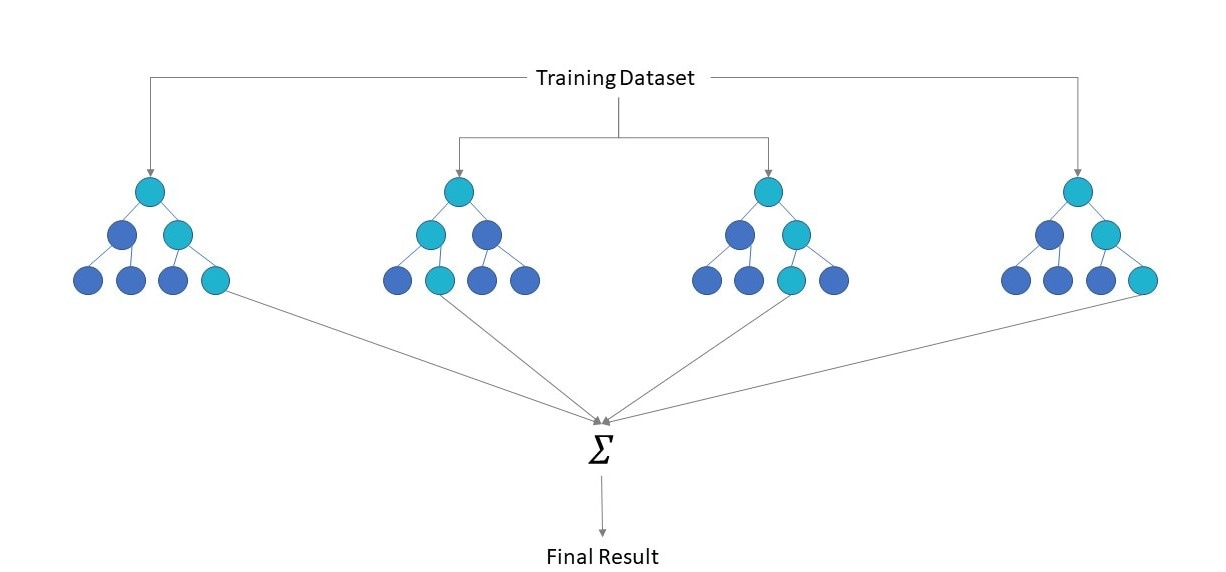
\includegraphics[width=0.5\textwidth]{chapters/contexto/images/rf.jpg}}
  \caption{\textmd{Abstração de uma Random Forest}}
  \legend{Fonte: What is Random Forest - IBM Cloud Education}
  \label{fig:rf-exemplo}
\end{figure}

\subsection{Gradient Boosting}
\label{subsec:contexto-gradient-boosting}

\textit{Machine Learning Boosting} é um método de criação de \textit{ensemble}s de classificadores, onde um modelo inicial é treinado com um conjunto de dados de treinamento, então um segundo modelo é construído com pesos nas predições erradas, de forma que a combinação deles resulte em um classificador melhor que ambos sozinhos, e esse processo é repetido por um número específico de instâncias ou até que o desempenho alcance um nível aceitável ou deixe de melhorar. As predições do \textit{ensemble} são combinadas, e a classe predita é a escolhida pela soma pesada das predições \cite{gb-towards}.

\textit{Gradient Boosting} é um tipo de \textit{Machine Learning Boosting}, onde \textit{Decision Tree}s são construídas de maneira aditiva e sequencial, uma de cada vez, sem alterar as árvores anteriores, e são julgadas por gradientes em uma função de perda, que serve como medida indicativa do seu desempenho. Um ponto positivo do \textit{Gradient Boosting} é que a sua função de perda é genérica e pode ser escolhida, permitindo que o algoritmo seja adaptado a diferentes tipos de problemas, como usar erro quadrático para regressão e perda logarítmica para classificação \cite{gb-mastery}.

\begin{figure}[ht!]
  \centering
  \fcolorbox{white}{white}{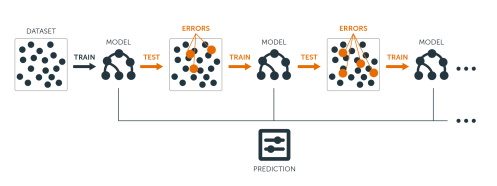
\includegraphics[width=0.5\textwidth]{chapters/contexto/images/gb.png}}
  \caption{\textmd{Abstração de Gradient Boosting}}
  \legend{Fonte: Hands-On Machine Learning with R (AI Wiki)}
  \label{fig:gb-exemplo}
\end{figure}

É possível configurar as árvores geradas da mesma forma que as \textit{Decision Tree}s, além de parâmetros como a taxa de aprendizado, servindo como um peso para cada adição, geralmente sendo um valor baixo entre 0,1 e 0,3, o que aumenta o número de árvores adicionadas ao modelo, diminuindo o impacto de cada árvore, mas deixando o modelo mais lento. Há também a possibilidade de utilizar \textit{Gradient Boosting} estocástico, utilizando subconjuntos de elementos ou atributos, diminuindo a correlação das árvores similar ao \textit{Random Forest}, mas com um custo computacional maior \cite{gb-mastery}.

\subsubsection{XGBoost}
\label{subsubsec:contexto-xgboost}

\textit{Extreme Gradient Boosting}, ou \textit{XGBoost}, é uma variação do \textit{Gradient Boosting} que, contrário à maneira sequencial do \textit{Gradient Boosting}, constrói as árvores paralelamente com uma estratégia por níveis, varrendo os valores de gradiente e usando as somas parciais como avaliação da qualidade de cada divisão possível. Há também várias outras otimizações de \textit{cache}, computação distribuída e adaptações para conjuntos de dados maiores que a capacidade de memória da máquina \cite{xgboost}.

\subsubsection{Light Gradient Boosting}
\label{subsubsec:contexto-light-gradient-boosting}

Outra variação do \textit{Gradient Boosting} é a sua versão mais leve, \textit{Light Gradient Boosting}, uma biblioteca de código aberto que busca ser mais eficiente e efetiva, muitas vezes alcançando essa visão até em conjuntos de dados de larga escala \cite{lgbm-mastery}. As diferenças vêm de um foco em gradientes maiores (\textit{Gradient-based One Side Sampling}) e a adição de uma seleção automática de características (\textit{Exclusive Feature Bundling}) \cite{lgbm}. Em certos casos, o \textit{Light Gradient Boosting} consegue uma pequena melhora na acurácia em relação ao \textit{XGBoost}, mas consegue ser até 7 vezes mais rápido \cite{lgbmvsxgboost}.

% \subsection{Rede Neural Artificial}
% \label{subsec:contexto-nn}

% \textit{Artificial Neural Network}, ou Rede Neural, é um algoritmo de classificação, agrupamento e regressão que se inspira no comportamento do cérebro humano, fazendo predições através de uma rede de neurônios.

% A Rede Neural é composta de camadas sequenciais de neurônios, começando por uma camada de entrada que recebe os dados, e terminando com uma camada de saída, que produz as predições, tendo uma quantidade configurável de camadas entre ambas, denominadas camadas ocultas.
% Cada neurônio pode realizar decisões matemáticas simples, sendo compostos por um vetor de entrada que possui pesos e viés, uma função de ativação e uma saída. Cada camada tem uma função de ativação, podendo ser configurada conforme a saída desejada para seus neurônios \cite{nn-image}. Considerando cada neurônio como um classificador por si próprio, a Rede Neural é um grande conjunto interconectado de classificadores que se alimentam sequencialmente \cite{nn-tds}.

% \begin{figure}[ht!]
%   \centering
%   \label{fig:nn-exemplo}
%   \fcolorbox{white}{white}{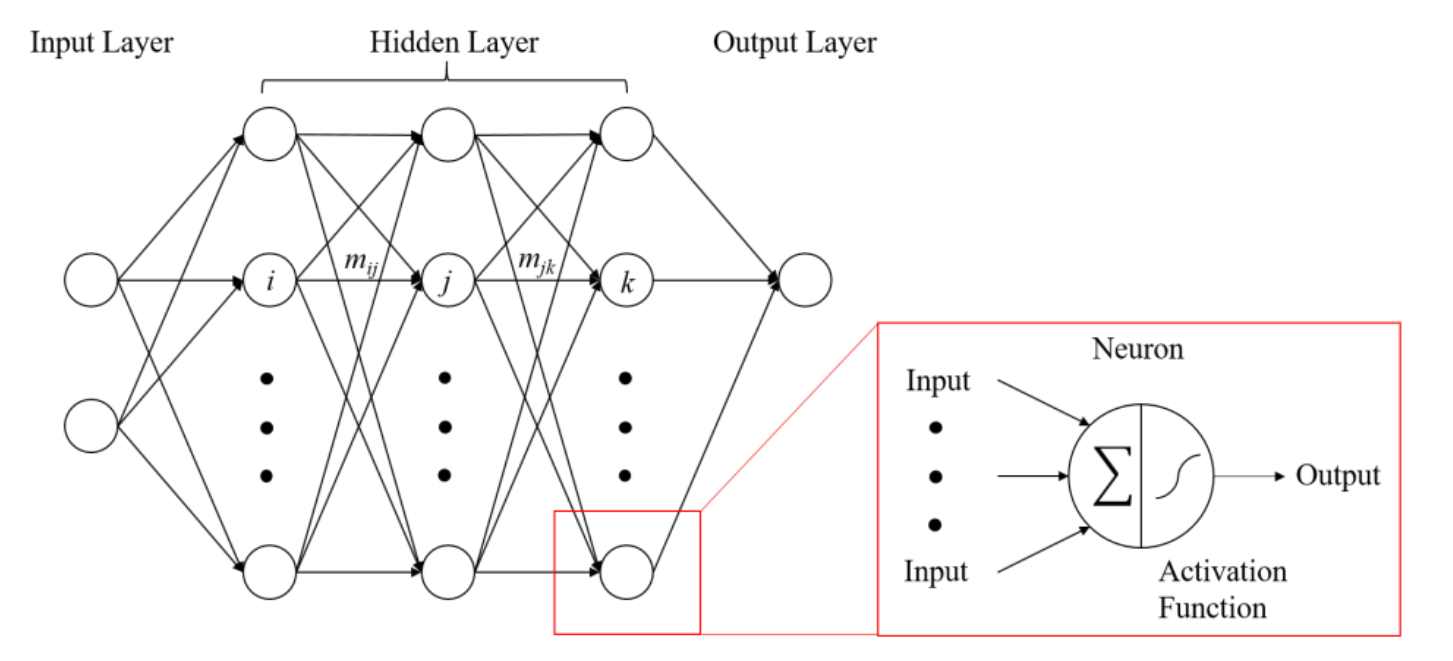
\includegraphics[width=0.8\textwidth]{chapters/contexto/images/nn.png}}
%   \caption{\textmd{Representação de uma Rede Neural Artificial}}
%   \legend{Fonte: \textit{Ensemble Neural Networks (ENN): A gradient-free stochastic method} \cite{nn-image}}
% \end{figure}

% A etapa de treinamento da Rede Neural consiste em definir uma função de perda e usar um algoritmo de otimização de gradiente descendente para encontrar os parâmetros da rede. Essa otimização é denominada \textit{backpropagation}, ou retropropagação, onde o erro encontrado pela função de perda é distribuído retrogradamente pela rede, onde cada neurônio aponta os neurônios acima dele que mais se ativaram. Esse processo possibilita que os pesos e viés de cada neurônio sejam ajustados corretamente \cite{nn-tds}.

% Redes Neurais possuem grande versatilidade, sendo utilizadas para resolver diversos problemas, como carros autônomos, reconhecimento facial, tradução, \textit{chatbots} e até produção de arte. Um problema comum, por outro lado, é a amplificação de viés já presentes nos conjuntos de dados, devido à sua forte identificação de padrões, sendo recomendado o uso de conjuntos de dados mais neutros.